\documentclass{standalone}

\usepackage[OT1]{fontenc}
\renewcommand*\familydefault{\sfdefault}
\usepackage{helvet,sfmath}
\usepackage{siunitx}

\usepackage{tikz}
\usetikzlibrary{arrows,calc,patterns}
% \usetikzlibrary{intersections, calc, arrows.meta}
\usepackage{tikz,tkz-euclide}

\begin{document}

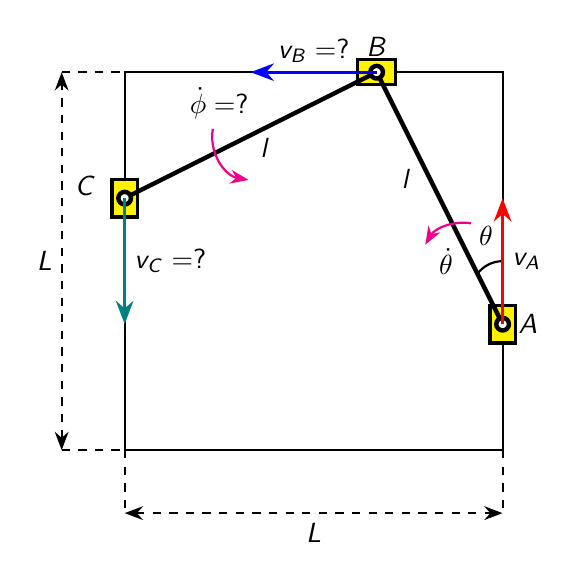
\begin{tikzpicture}[scale=0.8]
    \draw[thick] (0,0) rectangle (6,6);
    \draw[dashed, thick]
    (-1,0) to (0,0)
    (-1,6) to (0,6)
    (0,0) to (0,-1)
    (6,0) to (6,-1);
    \draw[dashed, thick, Stealth-Stealth] (-1,0) to (-1,6);
    \draw[dashed, thick, Stealth-Stealth] (0,-1) to (6,-1);
    \draw (3,-1) node[below]{\(L\)} (-1,3) node[left]{\(L\)};
    %% Bar
    \draw[fill=yellow, very thick] (5.8,1.7) rectangle (6.2,2.3);
    \draw[fill=yellow, very thick] (3.7,5.8) rectangle (4.3,6.2);
    \draw[fill=yellow, very thick] (-0.2,3.7) rectangle (0.2,4.3);
    \draw[ultra thick] (6,2) to (4,6) to (0,4);
    \draw (4.7,4.3) node[left]{\(l\)} (2,4.8) node[right]{\(l\)};
    \filldraw[color=black, fill=white, ultra thick](6,2) circle (0.1);
    \filldraw[color=black, fill=white, ultra thick](4,6) circle (0.1);
    \filldraw[color=black, fill=white, ultra thick](0,4) circle (0.1);
    \draw (6.1,2) node[right]{\(A\)} (4,6.1) node[above]{$B$} (-0.3,4.2) node[left]{\(C\)};
    \draw[thick] (6,3) arc (90:145:0.5);
    \draw (6,3.4) node[left]{\(\theta\)};
    %%
    \draw[very thick, red, -Stealth] (6,2) to (6,4);
    \draw[very thick, blue, -Stealth] (4,6) to (2,6);
    \draw[very thick, teal, -Stealth] (0,4) to (0,2);
    \draw (6,3) node[right]{\(v_A\)}
    (3,6) node[above]{\(v_B=?\)} 
    (0,3) node[right]{\(v_C=?\)};
    \draw[thick,magenta, -Stealth] (5.5,3.6) arc (80:150:0.7);
    \draw (5.1,3.0) node{\(\dot{\theta}\)};
    \draw[thick, magenta, -Stealth] (1.4,5.1) arc(170:260:0.7);
    \draw (1.5,5.5) node{\(\dot{\phi}=?\)};
\end{tikzpicture}

\end{document}
